\documentclass[10pt]{beamer}

\usepackage[utf8]{inputenc}
\usepackage{amsmath, amssymb, bm}
\usepackage{graphicx}
\usepackage{booktabs}
\usepackage{array}
\usepackage{multirow}
\usepackage{tikz}
\usepackage{appendixnumberbeamer}
\usetikzlibrary{positioning,arrows.meta,shapes.geometric}
\usepackage[style=authoryear,backend=biber,natbib=true,sorting=nyt]{biblatex}
\addbibresource{reference.bib}

\usetheme{Madrid}
\usecolortheme{default}
\setbeamertemplate{navigation symbols}{}
\setbeamertemplate{footline}[frame number]

\title[Preliminary Results]{Preliminary Empirical Results}
\subtitle{Testing the Zoning--Transportation Mechanism}
\author{Ke Jiang}
\institute{Southern Methodist University}
\date{\today}

\newcommand{\ubar}[1]{\underline{#1}}
\newcommand{\se}[1]{{\scriptsize(#1)}}

\begin{document}

\begin{frame}
  \titlepage
\end{frame}

%% ─────────────────────────────────────────────────────────────────────────────
\begin{frame}{Overview: Three Proposition Tests}

\begin{block}{Empirical chain from the model's FOC}
\begin{enumerate}
  \item \textbf{P1.} High employment concentration $\Rightarrow$ tighter residential zoning
  \item \textbf{P2.} Transit access raises population pressure $\Rightarrow$ tighter zoning response
  \item \textbf{P3.} Restrictive land use $\Rightarrow$ lower metropolitan transit investment
\end{enumerate}
\end{block}

\vspace{0.3cm}
\textbf{Data}
\begin{itemize}
  \item Tract-level housing supply elasticity $\hat{\gamma}_i$: \citeauthor{Baum-Snow2024-ii} (\citeyear{Baum-Snow2024-ii}), Dallas metro (N\,=\,1,016 tracts)
  \item Employment inflows $L_i$: LODES 2023, aggregated to Census tract
  \item Transit access: DART station locations (148 stations), 0.5-mile buffer
  \item Cross-metro zoning: WRLURI from Wharton; transit network: Transit Explorer (40 matched metros of 306)
\end{itemize}

\vspace{0.2cm}
\small\textit{Tests are equilibrium consistency checks, not causal estimates.
              Each proposition maps to a model FOC.}
\end{frame}

%% ─────────────────────────────────────────────────────────────────────────────
\begin{frame}[shrink=3]{P1: Employment Concentration and Zoning Restrictiveness}

\begin{columns}[T]
\column{0.44\textwidth}
\small
\textbf{Prediction.} From the municipal FOC,
\[
  \frac{\partial \hat\gamma_i}{\partial \log L_i} < 0.
\]
High-employment tracts face larger marginal congestion costs from looser zoning.

\vspace{0.25cm}
\begin{center}
  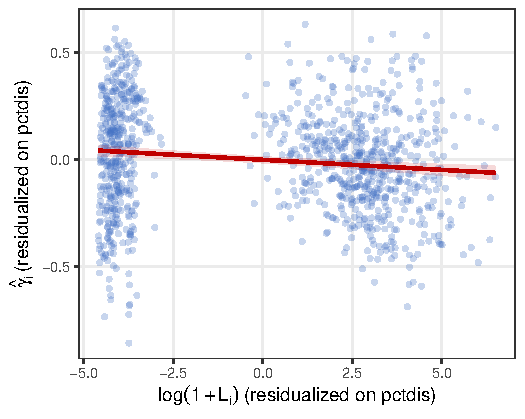
\includegraphics[width=\linewidth]{results/fig_p1_residualized.pdf}
\end{center}
{\scriptsize Residualized on CBD distance ($\widehat{\text{pctdis}}$).}

\column{0.56\textwidth}
\scriptsize
\resizebox{\linewidth}{!}{%
\begin{tabular}{lcccc}
\toprule
& (1) & (2) & (3) & (4) \\
& $\hat\gamma_{01a}$ & $\hat\gamma_{01a}$ & $\hat\gamma_{11a}$ & $\hat\gamma_{01a,\text{sp}}$ \\
\midrule
$\log(1+L_i)$
  & $-0.009^{***}$ & $-0.009^{***}$ & $-0.006^{***}$ & $-0.009^{***}$ \\
  & \se{0.002} & \se{0.002} & \se{0.002} & \se{0.002} \\[3pt]
$\text{pctdis}_i$
  & & $-0.087^{*}$ & $-0.095^{**}$ & $-0.040$ \\
  & & \se{0.045} & \se{0.045} & \se{0.042} \\[4pt]
\midrule
$R^2$ & 0.016 & 0.020 & 0.011 & 0.017 \\
$N$   & 1,016 & 1,016 & 1,016 & 1,016 \\
\bottomrule
\end{tabular}}

\vspace{0.2cm}
\normalsize
\begin{alertblock}{Result}
Negative and significant across all four specifications.
Consistent with the municipal congestion-cost FOC.
\end{alertblock}
\end{columns}

\end{frame}

%% ─────────────────────────────────────────────────────────────────────────────
\begin{frame}[shrink=5]{P2: DART Access and the Zoning-Tightening Response}

\begin{columns}[T]
\column{0.48\textwidth}
\small
\textbf{Prediction.} Transit access raises local attractiveness; municipalities respond
by tightening residential capacity:
\[
  \hat\gamma_i \big|_{\text{near DART}} < \hat\gamma_i \big|_{\text{far}}.
\]

\vspace{0.1cm}
\begin{center}
  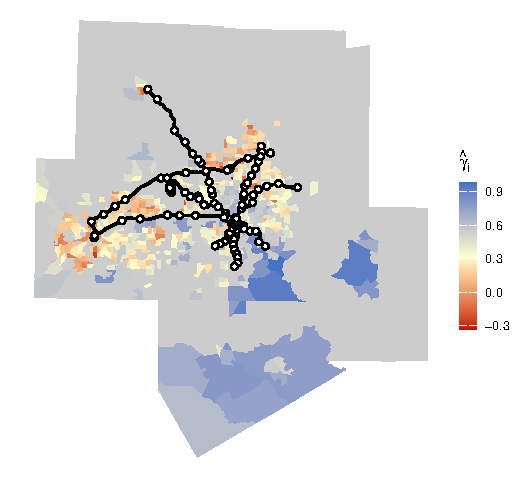
\includegraphics[width=\linewidth]{results/fig_p2_elasticity_map.pdf}
\end{center}
{\scriptsize Blue = high $\hat\gamma_i$ (permissive); red = low (restrictive). DART lines in black.}

\column{0.52\textwidth}
\scriptsize
\resizebox{\linewidth}{!}{%
\begin{tabular}{lcccc}
\toprule
 & (1) & (2) & (3) & (4) \\
\midrule
$\mathbf{1}[\text{near DART}]$
  & $-0.152^{**}$ & $-0.205^{***}$ & $-0.178^{***}$ & $-0.177^{**}$ \\
  & \se{0.059} & \se{0.058} & \se{0.057} & \se{0.079} \\[3pt]
$\text{pctdis}$
  & & $-0.412^{***}$ & $-0.384^{***}$ & $-0.384^{***}$ \\
  & & \se{0.059} & \se{0.059} & \se{0.059} \\[3pt]
$\log(1+L_i)$
  & & & $-0.032^{***}$ & $-0.032^{***}$ \\
  & & & \se{0.007} & \se{0.007} \\[3pt]
$\mathbf{1}[\text{near}]\times\text{pctdis}$
  & & & & $-0.011$ \\
  & & & & \se{0.418} \\[3pt]
\midrule
$R^2$ & 0.011 & 0.087 & 0.118 & 0.118 \\
$N$   & 581   & 581   & 581   & 581   \\
\bottomrule
\end{tabular}}
\vspace{0.15cm}
{\scriptsize N\,=\,581 Baum-Snow tracts matched to 2020 Census geometry; 15 have DART-adjacent centroid.}

\vspace{0.1cm}
\normalsize
\begin{block}{Result}
Near-DART tracts have elasticities 0.18 units lower.
Interaction insignificant (few suburban near-station tracts).
\end{block}
\end{columns}

\end{frame}

%% ─────────────────────────────────────────────────────────────────────────────
\begin{frame}[shrink=5]{P3: Zoning Restrictiveness and Metro Transit Networks}

\begin{columns}[T]
\column{0.48\textwidth}
\small
\textbf{Prediction.} Restrictive zoning suppresses ridership density, lowering transit ROI:
\[
  \frac{\partial \log(\text{TransitKm}_m)}{\partial \text{WRLURI}_m} < 0.
\]

\begin{center}
  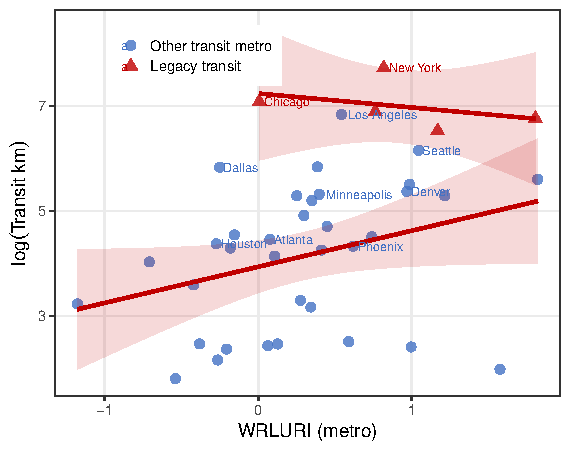
\includegraphics[width=\linewidth]{results/fig_p3_wrluri_transit.pdf}
\end{center}
{\scriptsize 40 US metros with existing transit matched to Baum-Snow; red = legacy systems.}

\column{0.52\textwidth}
\scriptsize
\resizebox{\linewidth}{!}{%
\begin{tabular}{lccccc}
\toprule
& \multicolumn{3}{c}{All metros ($N$=306)} & \multicolumn{2}{c}{Transit only} \\
\cmidrule(lr){2-4} \cmidrule(lr){5-6}
& (1) & (2) & (3) & (4) & (5) \\
\midrule
WRLURI
  & $0.538^{***}$ & $0.193^{*}$ & $0.196^{*}$ & $0.965^{***}$ & $0.849^{**}$ \\
  & \se{0.119} & \se{0.100} & \se{0.101} & \se{0.284} & \se{0.332} \\[3pt]
$\log(\text{tracts})$
  & & $0.847^{***}$ & $0.844^{***}$ & $0.995^{***}$ & $0.731^{**}$ \\
  & & \se{0.068} & \se{0.068} & \se{0.208} & \se{0.271} \\[3pt]
FracUnavail
  & & & $-0.147$ & & $0.285$ \\
  & & & \se{0.431} & & \se{1.413} \\
\midrule
Legacy excl.? & -- & -- & -- & No & Yes \\
$R^2$ & 0.063 & 0.383 & 0.383 & 0.484 & 0.274 \\
$N$   & 306   & 306   & 306   & 40    & 35    \\
\bottomrule
\end{tabular}}

\vspace{0.1cm}
\normalsize
\begin{alertblock}{Sign reversal — caution}
\small WRLURI is \emph{positive}: coastal legacy metros (NY, SF, Boston)
are both more restrictive \emph{and} have larger transit systems.
This reflects historical endogeneity, not a refutation of the model.
\end{alertblock}
\end{columns}

\end{frame}

%% ─────────────────────────────────────────────────────────────────────────────
\begin{frame}[shrink=5]{Interpretation and Next Steps}

\begin{columns}[T]
\column{0.5\textwidth}
\begin{block}{What the tests show}
\begin{itemize}\small
  \item \textbf{P1 \checkmark} Employment-concentrated tracts are systematically less permissive, consistent with the municipal congestion-cost FOC.
  \item \textbf{P2 \checkmark} DART-adjacent tracts are significantly less permissive than matched non-adjacent tracts, consistent with the transit-tightening channel.
  \item \textbf{P3 —} Cross-metro raw correlation is \emph{positive}: legacy transit cities are restrictive and transit-rich. Historical endogeneity prevents direct inference.
\end{itemize}
\end{block}

\column{0.5\textwidth}
\begin{alertblock}{Identification strategy needed for P3}
\begin{itemize}\small
  \item Control for pre-automobile urban form (1920 density)
  \item Instrument WRLURI with state-level regulation history or terrain
  \item Use planned-but-unbuilt lines to isolate transit supply variation
  \item Restrict to metros without pre-war rail (cleaner counterfactual)
\end{itemize}
\end{alertblock}

\vspace{0.2cm}
\begin{block}{P2 refinements}
\begin{itemize}\small
  \item Expand to other metros in Baum-Snow sample
  \item Use distance to nearest station (continuous)
  \item Historical station-siting instrument for causal test
\end{itemize}
\end{block}
\end{columns}

\end{frame}

%% ─────────────────────────────────────────────────────────────────────────────
\begin{frame}{Summary}

\centering
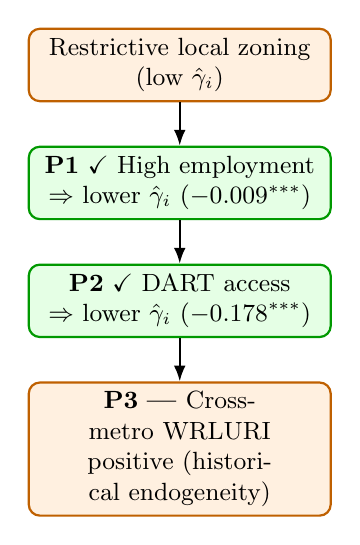
\begin{tikzpicture}[
  node distance=0.55cm and 0.3cm,
  box/.style={rectangle, rounded corners, draw=blue!65, fill=blue!8, thick,
              align=center, minimum height=0.55cm, text width=3.6cm, font=\small},
  res/.style={rectangle, rounded corners, draw=green!60!black, fill=green!10, thick,
              align=center, minimum height=0.55cm, text width=3.6cm, font=\small},
  warn/.style={rectangle, rounded corners, draw=orange!75!black, fill=orange!12, thick,
               align=center, minimum height=0.55cm, text width=3.6cm, font=\small},
  arrow/.style={-{Latex[length=2mm]}, thick}
]
\node[warn] (z)    {Restrictive local zoning\\(low $\hat\gamma_i$)};
\node[res,  below=of z] (e) {\textbf{P1 \checkmark} High employment\\$\Rightarrow$ lower $\hat\gamma_i$ ($-0.009^{***}$)};
\node[res,  below=of e] (t) {\textbf{P2 \checkmark} DART access\\$\Rightarrow$ lower $\hat\gamma_i$ ($-0.178^{***}$)};
\node[warn, below=of t] (p) {\textbf{P3 —} Cross-metro WRLURI\\positive (historical endogeneity)};

\draw[arrow] (z) -- (e);
\draw[arrow] (e) -- (t);
\draw[arrow] (t) -- (p);
\end{tikzpicture}

\vspace{0.3cm}
\small
P1 and P2 provide within-DFW equilibrium support for the model's municipal FOC.\\
P3 requires causal identification via historical or geographic instruments.

\end{frame}

\end{document}
